% 2009 年上海卷理科第 5 题：题图。
% 来源 PDF：普通高考/2009/2009上海理.pdf，SHA256 82ede013bf354097cfc65c1bab2885db813572321b6eb0012f445c1c754d3fa8
% 原页：第 1 页（A3 三栏）第 1 栏，印刷页 553。
% 重绘依据：正四棱柱底面边长 2、高 4，B-D_1 虚线，AD 为底边；与文科同题一致。
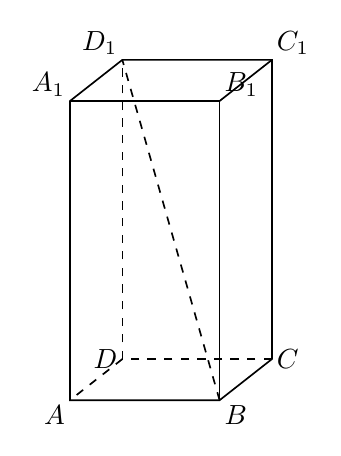
\begin{tikzpicture}[scale=0.95, semithick, every node/.style={inner sep=1.5pt}]
  \coordinate (A)  at (0,0);
  \coordinate (B)  at (2,0);
  \coordinate (D)  at (0.7,0.55);
  \coordinate (C)  at (2.7,0.55);
  \coordinate (A1) at (0,4);
  \coordinate (B1) at (2,4);
  \coordinate (D1) at (0.7,4.55);
  \coordinate (C1) at (2.7,4.55);
  \draw[dashed] (D) -- (D1);
  \draw[dashed] (C) -- (D);
  \draw[dashed] (D) -- (A);
  \draw (A) -- (B) -- (C) -- (C1) -- (D1) -- (A1) -- cycle;
  \draw (A) -- (A1);
  \draw (B) -- (B1);
  \draw (C) -- (C1);
  \draw (B1) -- (C1);
  \draw (A1) -- (B1);
  \draw[dashed] (B) -- (D1);
  \node[anchor=north east] at (A)  {$A$};
  \node[anchor=north west] at (B)  {$B$};
  \node[anchor=west]       at (C)  {$C$};
  \node[anchor=east]       at (D)  {$D$};
  \node[anchor=south east] at (A1) {$A_1$};
  \node[anchor=south west] at (B1) {$B_1$};
  \node[anchor=south west] at (C1) {$C_1$};
  \node[anchor=south east] at (D1) {$D_1$};
\end{tikzpicture}
